\documentclass[11pt,letterpaper]{article}
\usepackage[top=1.00in, bottom=1.0in, left=1in, right=1.25in]{geometry}
\usepackage{graphicx}
\usepackage{latexsym,amssymb,epsf}
\usepackage{epstopdf}

\usepackage{sectsty,setspace,natbib}
\usepackage{float}
\usepackage{latexsym}
\usepackage{hyperref} 
\usepackage{hyperref}
\usepackage{epsfig}
\usepackage{graphicx}
\usepackage{amsmath}
\usepackage{array}
\usepackage{lineno}
\usepackage{gensymb}

\usepackage{todonotes}
\usepackage{framed}

\linespread{1.1} % was 1.66 for double-spaced 
% \raggedright
\setlength{\parindent}{0.5in}
\pagestyle{empty}

\parskip=5pt
\pagenumbering{arabic}
\pagestyle{plain}
\setlength\parindent{0pt}

\begin{document}
\begin{flushright}
Version dated: \today
\end{flushright}
\bigskip
\noindent RH: Environmental tracking 
% put in your own RH (running head)
\bigskip
\medskip
\begin{center}
% Insert your title:
\noindent{\Large {\bf How environmental tracking shapes communities in stationary \& non-stationary systems}}\\
% Other titles: `Environmental tracking: It's more complicated than you think' (we hope) 
% or `Environmental tracking: Is it naive? Or, are we just naive?'
\bigskip
\noindent {\normalsize
E. M. Wolkovich$^{1}$ \& M. J. Donahue$^{2}$ }\\
\noindent {\small \it
% $^1$ Arnold Arboretum of Harvard University, 1300 Centre Street, Boston, Massachusetts, 02131, USA\\
% $^2$ Organismic \& Evolutionary Biology, Harvard University, 26 Oxford Street, Cambridge, Massachusetts, 02138, USA\\
$^1$ Forest \& Conservation Sciences, Faculty of Forestry, University of British Columbia, 2424 Main Mall, Vancouver, BC V6T 1Z4\\
$^2$ Hawaii Institute of Marine Biology, University of Hawaii at Manoa, Kaneohe, HI 96744}\\
\medskip
\end{center}
\noindent{\bf Corresponding author:} XX, see $^{1,2}$ above ; E-mail:.\\

\newpage
%\linenumbers

\begin{abstract} 
Climate change is reshaping the environments of all species. Predicting how communities will shift in the face of this change requires understanding the mechanisms that govern how communities assemble, and how such mechanisms will shift with warming. Growing empirical evidence suggests that environmental tracking is linked to species performance, and thus may be a structuring force in communities today. Here, we review current knowledge on temporal environmental tracking both in empirical data and through the lens of fundamental community ecology theory. Focusing on how climate change has altered the start of the growing season, we provide an initial test of how well basic theory supports the paradigm that climate change should favor environmental tracking. We then show how non-stationary environments may fundamentally alter these conclusions and the mechanisms that structure ecological communities. Finally we review how the reality that change has and is expected to affect far more than mean temperatures, including widespread affects on growing season length, variability and shifts in extreme events may complicate simple predictions of winners and losers with climate change. 
% 175 words
% Finally, we provide a framework to leverage existing ecological theory to understand how tracking in stationary and non-stationary systems may shape communities, and thus help predict the indirect consequences of climate change.
% % Climate change upends the assumption of stationarity. By causing increases in temperature, larger pulses of precipitation, increased drought, and more storms \citep{ipcc2013}, climate change has fundamentally shifted major attributes of the environment from stationary to non-stationary regimes.
\end{abstract}
\noindent \emph{Keywords:} phenology, climate change....\\



\section{Main text}
Anthropogenic climate change causes widespread changes in species distributions, with many species shifting in both time and space \citep{IPCC:2014sm}. Reports often focus on species shifting to higher elevations and poleward \citep{Chen2011}, and/or shifting their recurring life history events (phenology) earlier as climate warms \citep{Menzel:2006sq,Wolkovich:2012n,cohen2018}. A large proportion of species, however, are shifting much less \citep{Cook:2012pnas}, raising concerns about whether these species may be more vulnerable to population declines with continued warming. Such conclusions come in part from increasing research that links how well species track climate change---especially through temporal shifts---to shifts in biomass, growth and other metrics related to performance \citep{Cleland:2012}. Tracking may then be a major component to understanding and predicting indirect effects of climate change---including population declines, with cascading effects on community and ecosystem structure.

How well a species tracks the environment through its phenology has repeatedly been linked to other species' responses to climate change \citep{Cleland:2012,ramula2015}. Species that phenologically track warming appear to perform better in field warming experiments \citep{Cleland:2012}, and exotic plant species appear to gain a foothold in warming environments by phenologically tracking climate change \citep{Willis:2010al}. Simple community ecology theory supports these findings, suggesting that a warming climate should open up new temporal niche space and favor species that can exploit that space \citep{gotelli1996,wolkovich:2010fee,Zettlemoyer2019}. Thus, a shift toward earlier spring should favor earlier species, especially those that can environmentally track ever-earlier seasons. This hypothesis has gained significant traction in the ecological literature focused on global change \citep[e.g.,][]{Cleland:2012}; however, there has been comparatively little work examining whether it is supported through coexistence theory and models. 

Current or `modern' coexistence theory is based strongly on understanding how variable environments may promote coexistence---providing one way to study how communities may be shaped by a temporally varying environment and how tracking may allow a species to take advantage of that variability. Most theory, however, is based on the assumption of stationarity: though the environment is variable, its underlying distribution is unchanged across time \citep{barabas2018}. This assumption is common not just to coexistence theory, but to much of the theory that underlies ecology, evolution, and myriad other research fields \citep[e.g.,][]{Milly:2008yu,nosenko2013}. 

Climate change upends the assumption of stationarity. By causing increases in temperature, larger pulses of precipitation, increased drought, and more storms \citep{ipcc2013}, climate change has fundamentally shifted major attributes of the environment from stationary to non-stationary regimes. This transition is reshaping ecological systems, and, while new work has aimed to adapt coexistence to non-stationary environments \citep{chessonnonstat}, little work has examined what such a transition may mean for communities and the species within them.  % Importantly, models based on the theory can help highlight which species `traits,' including those related to how species are matched to and respond to the environment, are favored under different environmental regimes.

Here, we review current knowledge on temporal environmental tracking both in empirical data and through the lens of basic community ecology theory, highlighting where simple theory predicts complexities often seen in empirical results. We review current coexistence theory for variable environments and provide an initial test of how well basic theory supports the current paradigm that climate change should favor species with environmental tracking. Finally, we provide a framework to leverage existing ecological theory to understand how tracking in stationary and non-stationary systems may shape communities, and thus help predict the indirect consequences of climate change. 

\subsection{Environmental variability \& change}

Decades of ecological research highlight how variable environments shape species and their communities at multiple scales \citep{Sale:1977oq,Chesson:1997dz}.  In seasonal landscapes, the environment limits periods for growth each year (e.g., by temperature or drought); within-year variability in the environment (e.g., daily, hourly or finer resolution temperatures or rainfall amounts) compounds into inter-annual variability that shapes the distrubution of the start and end of growing seasons. For long stretches of history this variability has been stationary; that is, the underlying probability distribution that describes the start (or end) of the season (e.g., the date of the last major frost) does not change, even though the date may be dramatically different from one year to the the next (i.e., each year is a single draw from the distribution). The shape of this underlying distribution varies across systems and in how it is measured---for example, the total amount of rainfall across years in semi-arid systems is often highly skewed (rare high rainfall years, with many more below-average rainfall years) compared to the more normal distribution of the thermal sum of many temperate growing seasons. 
% In seasonal landscapes, periods for growth each year are limited (e.g., by temperature or drought), and species must manage within-year variability by timing when to grow and when to reproduce \citep{donohue2002}. 

In other time periods, variability is non-stationary in one or multiple dimensions. For example, climate in the northern hemisphere includes long warming and then cooling periods (i.e., increasing then decreasing means of the probability distribution) at the start of the Holocene, when the earth was coming out of the last glacial maximum. Anthropogenic climate change (henceforth, referred to simply as `climate change') is a similar non-stationary process, with warming evident around the globe and knock-on effects for other climate metrics, such as heat extremes and the size of precipitation events. While only several decades ago, ecology was focused strongly on stochasticity in stationary systems \citep[e.g.,][]{Ripa1996,Kaitala1997}, climate change has shifted the focus to understanding stochasticity in a non-stationary framework \citep[e.g.,][]{cazwavelets,ehrlen2016}.

Understanding non-stationarity in ecological systems requires first identifying which aspects of the environment have shifted---and how they have shifted with respect to one another---as the underlying distributions transition from stationary to non-stationary. For example, with climate change, warming has increased mean tempertures over time, with minimum temperatures generally increasing more than maximum---this results in an underlying distribution for daily temperature where the mean is increasing through time and the variance is decreasing \citep{ipcc2013,screen2014}, despite a growing literature on increasing variance in temperature \citep[e.g.,][]{vasseur2014}. In many systems, climate change has altered aspects of the environment relevant to species timing (Fig. \ref{fig:climdat}).

\subsection{Environmental tracking in time}

Environmental variability means many species should benefit from tracking their environment. We focus here on environmental tracking through time (often referred to below as `tracking') rather than through space because of its well-established links to individual-level physiology, yielding a more robust understanding of what environmental cues determine tracking \citep{chuineJTB,Chew:2012pd}, and because it has been repeatedly linked to performance and other fitness-related metrics. Temporal environmental cues, however, are often linked to species' ranges \citep{Morin:2008vp,arabid2011}, thus we expect much of this work could extend to environmental tracking through space. 

Most species track their environments through time by adjusting their phenologies, but identifying this tracking depends on many factors (see Box). Many (or potentially all) species for example use abiotic cues to trigger major phenological events. These cues in turn result in different rates of tracking. At one extreme, some cues yield a fixed timing that is consistent every year (which, on an inter-annual scale would be observed as no tracking). A common example of a fixed cue is photoperiod, which results in event timing that is constant across years (but variable across space, allowing---for example, later timings poleward for spring events) and appears prevalent in some insect emergence and for fall senensence of many trees \citep{Denlinger2017,lechowiczbook2002}. Fixed timings are pehaps the simplest option, and may be an efficient option for events where there is low variability or low costs to being too late or early. In cases where there is a high cost to mis-timing an event across a variable environment, cues related to climate are far more prevalent. Temperature is a widespread cue for start of season events, with many organisms needing a certain thermal sum to start visible growth. Such a cue has the benefit of shifting the date of an event early or late, depending on climatic conditions, each year, but may be a poor cue in years with aberrant late frost events. In most systems, species must use cues to forecast the ideal start of season date---a date which is only obvious in retrospect. 

Not surprisingly, simple environmental metrics are almost always proxies for a more complicated underlying physiology where simple cues---such as those to warm temperatures---can be modified by other cues, such as photoperiod, drought or light spectra \citep{Bagnall1993,Stinchcombe:2004ec}. These additional cues almost always appear designed to handle unusual---though not completely uncommon---years when the simple cue alone would fail---that is, would trigger growth, reproduction or another life history event at a highly suboptimal time. For example, in many temperate forest systems, woody plants cue strongly to warm spring temperatures, but also to cool winter temperatures, which prevents leafout in warm snaps that occur in many climates in the middle of the winter---long before the last risk of frost damage is past. In some semi-arid systems, species time growth to pulses of rain, but only when those rain events occur with cooler temperatures, that indicate the start of the rainy season, and not a rare summer rainfall event in the middle of months of drought \citep{Wainwright:2012tw,wainwright2013}.  % Process-based models can help include some of these complexities, especially when informed by observational and experimental results, but even for such well studied systems as \emph{Arabidopsis thaliana} there is still some noise in predictions versus empirical results. 

%  All these approaches  are focused on the proximate level---what environmental cues underlie tracking---at the ultimate level tracking is shaped by what resources species need to grow and reproduce. 
The complexities of cues underlying environmental tracking highlight that, at the ultimate level, tracking is shaped by complex resources that species need to grow and reproduce. This is perhaps best recognized in the literature on trophic synchrony where focus is often on how well consumers track their prey resources \citep{deacy2018,kharouba2018}. For example, decades of work has studied how birds (e.g., \emph{Parus major}) time their peak food demands---during their nesting season---to maximal prey (caterpillar) abundance \citep[e.g.,][]{charm2008}. Failure to track prey year-to-year or over time with warming has been well tied to individual-level fitness consequences in some systems \citep{charm2008}, but not all \citep{visser2006}. Tracking of plants and other lower trophic levels is also equally about resources. Alpine plant species that emerge in step with snowmelt are likely responding, at least in part, to light resources for photosynthesis. Light equally appears critical to the sequence of phenology in many temperate forests: with lower-canopy species, and younger (shorter) individuals of higher-canopy species, routinely risking frost damage to leafout before the canopy closes and access to light becomes severely reduced \citep{Vitasse2013,heberling2019}. In both temperate as well as alpine systems, however, access to critical belowground resources also occurs in the spring---both for available water but also for nutrients released with the turnover of seasonal microbial communities \citep{Zak:1990ar}. Thus, plants' spring phenology in many systems is about careful tracking to optimally compete for nitrogen and other soil resources. As in higher trophic level systems, research has linked how well plants track to performance, with species that track warming more tending to grow larger and/or produce more offspring \citep{Cleland:2012}.

\subsection{Interspecific variation in tracking}
% ADD  some numbers on variation in tracking ... why the variation? (1) it's hard to measure (keep this quick? Reference box?) and (2) maybe it's not always optimal to track ... boom, coexistence theory to the rescue!
Despite the clear importance of tracking for resource access, not all species appear to track their environments equally well \citep{thackeray2016}. Many plant species track spring temperatures strongly \citep[multiple meta-analysis now show plants's spring phenology on average track spring or annual temperatures 4-6 days/$\degree$C][and simple temperature models can often explain over 90\% of interannual variation in phenology]{Richardson:2006qh,Wolkovich:2012n,thackeray2016}, but other species do not \citep{Cook:2012pnas} and do not appear linked to other major climate variables \citep{thackeray2016}. Variability equally exists when examining consumers tracking their prey \citep[across diverse species tracking over time is 6.1 days/decade but ranges from zero to 15 days/decade, see][]{kharouba2018}. Such variation in tracking across taxa is driven in part by difficulties in measuring tracking (see Box). Yet other variation may be real and suggests perfect environmental tracking may either not be possible or optimal for all species. 

Within populations, life-history can help predict how much individuals should track while also balancing trade-offs within and across seasons and years. Tracking has been repeatedly linked to fitness benefits \citep[e.g.,][]{farzan2018,deacy2018}. Such benefits usually break down into avoiding tissue loss or maximizing growth and, relatedly, maximizing reproduction. Species often track the start of growing seasons to avoid substantial tissue loss, for example from frost damage in temperate plants, or start activity only when resources for growth are present, such is the case in animals coming out of hibernation in cold regions. Equally, tracking of resources throughout a season is linked to the timing of reproduction for many species and, for iteroparous species, decisions on how much to invest each season requires estimating how likely a year is to be good for offspring. For species with bounded growing seasons, much literature has reviewed how tracking is a multivariate equation balancing early-season access to resources and its associated risks of tissue loss, with later season tracking of resources for reproduction and time for offspring to mature \citep{donohue2002,Morin:2005ye,Burghardt2015}. These trade-offs should also scale up to predictions of variation in tracking across species. 

Across species, community ecology theory makes predictions for suites of traits that may trade-off with tracking. As tracking fundamentally relates to tracking a resource pulse in most systems, traits related to resource use are likely contenders for a trade-off. Species with traits that make them poor resource competitors may need to track the environment closely, while superior competitors could outcompete trackers, and thus hypothetically track the environment less closely. Examples include under-canopy species leafing out earlier to gain access to light \cite{pheberling2019} or plants with shallow roots starting growth sooner in semi-arid systems, while species with deeper roots may begin growth later \citep{Zhu2016BioLetters}. In such cases, tracking is akin to a competition-colonization trade-off \citep{Amarasekare:2003tq}, where species that track well gain priority access to resources and, thus, may co-exist with superior competitors. 

% Need to update below after minimeta is done!
Research on phenological tracking and traits has increased greatly in recent years, with a major uptick in studies after 2010 (see Supp Fig. S1). Of 176 papers we found using terms related phenological tracking and traits 82\% were published in 2011 or later. Despite increasing interest in this topic, very few papers actually evaluated relationships between tracking and traits (13 papers, see Supp for more details), with most lacking data on one aspect of the relationship or the other (102 papers), some focusing on intraspecific variation (32 papers), and others discussing links and having relevant data, but providing no robust statistical tests (X studies). Of the few studies that did link tracking and traits, most were on plants (9 papers), with three on butterflies and one on birds. By far the most studied trait was how early or late a phenophase occurred (e.g., date of flowering of start of migration for a species, termed `earlyness' by some authors), with earlier species tending to track more. While this is an important link it is vulnerable to statistical challenges (see Box). Few studies examined whether tracking correlates with resource aquisition traits, though those that did examine such traits generally found species with higher tracking also had traits associated with lower competitve abilities under low resources (e.g., shallower rooted). The link between tracking and `earlyness,' if robust, may provide a further link to resource aquisition traits as previous work has documented that species with earlier phenophases tend to have traits associated with lower competitve abilities \citep[e.g., they tend to be of lower height, have shallower roots, narrower diameter vessels, thinner leaves, and grow faster,][]{wolkovich2014aob}. 
% Earlyness is the average tauIhat ... 
% ii. Links to trait literature? Not enough study of traits that include tracking components (because that’s hard)
%      A. how much do people look at trade-offs?
%      B. phenology can impact traits themselves, so how to analyse (competition experiments?)

These trade-offs with tracking, predicted by basic ecological theory and tentatively supported by growing empirical work, would have fundamental consequences for community assembly, especially with climate change. Applying this ecological theory to current environments, however, is difficult because most theory has been developed for stationary systems \citep[as is the case in other sciences, ][]{Milly:2008yu}, which are mathematically more tractable, and can sometimes be extended to non-stationary systems \citep{chessonnonstat}. Almost no community assembly research, however, has examined the consequences of shifting from a stationary to non-stationary environment. Yet this transition is exactly what anthropogenic climate change has imposed on systems around the globe, making our understanding of how environmental tracking fits within community assembly theory critical. 
% .... that would have fundamental consequences for community assembly---at least in stationary systems. In non-stationary systems, theory is less developed for how tracking may trade-off with other traits (CITECHESSON), and even less theory predicts the consequences if the environment shifts from stationary to non-stationary

% How to explain warming experiments where researchers have identified links between performance and tracking, 
% links between tracking and performance in warming experiments could potentially wash out over longer timescales (fitness not measured over long enough timescales to consider diverse species life history strategies)

% consider cost of static timing (cheap) versus tracking (potentially costly)
% Variation in tracking may also be predicted based on historical effects ... change in environment (species track old environment)

\subsection{The role of the environment in coexistence} % or Coexistence theory \& environmental tracking 
Recent advances in coexistence models, often heralded under the title `modern coexistence theory,' recognize that both mechanisms independent of fluctuations in the environment (e.g., R* and other classical niche differences) and dependent on fluctuations in the environment (relative non-linearity and storage effect) can drive coexistence \citep{Chesson:1997dz,Chesson:2000vd}. Models under this paradigm are thus often composed of parameters that the describe the environment and the species within it (Megan--suggest CITES [working on it]). Parameters related to species must always include mechanisms for growth, death, interactions with other species, and generally a bet-hedging strategy for survival across years (e.g., a seedbank or other long-lived lifestage)---though exactly how these are defined varies across models (e.g., R* and related models focus on resource competition). 

How the environment is defined in most models falls into two broad categories. In some models the environment is expressed as variation in parameters related to species (e.g., in some lottery models the environment appears, effectively, as variation in birth and death rates). In other models, the environment is more specifically defined. For example, many seed germination models define an environment that begins with a resource pulse each year. Building a changing environment into models thus may require knowing how environmental shifts filter through to species-level parameters \citep{Tuljapurkar2009} or---perhaps more simply---how the environment is changing. In the aforementioned seed germination models for example, many systems may be experiencing shifts in the size or variability of the resource pulse. 
%[I like how this is framed, but  what is coming to mind for me is the idea of the environment coming into models as "species response to the environemnt", and not the environment itself.  This is the lottery model example you provide.  In some ways, our model takes both approaches - the germination function is more a a species response to envt - it essentially defines how a species responds to a particular tauP - but the resource level is, itself, the level of thresource in the system,. So our between year effects are species-response to envt and within year are more actual envt.  I'm not sure this is a helpful comment...]
% \citep{Davison2010,morris2008,Tuljapurkar2009}
% Lottery model: Birth and death rates vary ... collapses to single ratio (that's the environment) ... many general models are like this, they just vary a parameter and assume it is varying in response to the environment. Whatever parameter you allow to vary is how you allow the environment to filter through. (Side note: Tulja Purqur may have worked on how environment filters through to many species parameters in the model.)

These models, which underlie much of current community ecology research \citep{Mayfield:2010fe,barabas2018,ellner2019}, allow tests of basic predictions of how tracking may shape communities. While growing empirical research supports that tracking is an important trait---especially in a changing environment---there are few tests of whether models support these basic theoretical predictions. Below we examine how tracking may shape communities in stationary environments and environments transitioning from stationary to non-stationary.

\subsubsection{Model description}
% To understand the role of environmental tracking by species in variable environments 
We use a simple model that includes dynamics at both the intra-annual and inter-annual scales. As the model is akin to many commonly used seed germination models \citep{Chesson:2004eo}, we follow a similar terminology for ease; however the basic structure of our model could apply to others systems with one dominant pulse of a limiting resource each season (e.g., water from rain or snowpack).  This model thus allows within- and between-year dynamics to contribute to coexistence. Between-years the environment is included via variable germination, and within-years the environment is explicitly included as a resource pulse at the start of the season. The model includes a suite of species traits; of interest here, are traits controlling species response to the environment via germination each year, traits related to how species may bet-hedge across years (via a seedbank), as well as traits relating to resource competition each year. Within-season dynamics are controlled by resource competition resulting in fitness diffferences, while interannual variation in the environment provides opportunities for coexistence via fluctuation-dependent mechanisms (i.e., niche differences resulting from different germination functions). 

Across years, for a community of \(n\) species, the seedbank ($N$) of species $i$ at time $t+1$ is determined by the survival ($s_i$) of seeds that did not germinate in season t ($1-g_{i}(t)$) plus new biomass ($B_i$) produced during the length of the  growing season ($\delta$) converted to seeds ($\phi_i$):
\begin{align}
N_{i}(t+1) & =
s_{i}N_{i}(t)(1-g_{i}(t))+\phi_{i}B(t+\delta)
\end{align}
The production of new biomass each season follows a basic R* competition model: new biomass production depends on its resource uptake ($f_i(R)$ converted into biomass at rate $c_i$) less maintenance costs ($m_i$), with uptake controlled by $a_i$, $u_i$, and $\theta_i$:
%[I don't think that dB/dt should be a partial differential, but the same as dR/dt]
\begin{align}
\frac{\mathrm{d}B_i}{\mathrm{d}t} & = [c_{i}f_{i}(R) - m_{i}]B_{i} \\
f_{i}(R) & = \frac{a_{i}R^{\theta_{i}}}{1+a_{i}u_{i}R^{\theta_{i}}}
\end{align}
With the initial condition:
\begin{align}
B(t+0) & = N_{i}(t)g_{i}(t)b_{0,i}
\end{align}
where b0 is the inital biomass per seed.
The resource ($R$) itself declines across a growing season due to uptake by all species and abiotic loss ($\epsilon$):
\begin{align}
\frac{\mathrm{d}R}{\mathrm{d}t} & = - \sum_{i=1}^{n}f_{i}(R)B_{i} -\epsilon R
\end{align}
Germination depends the germination traits of the species and on the environment that year. The fraction of seeds germinating each year for a species is determined by the distance between $\tau_i$, a species characteristic, and $\tau_P$, an attribute of the environment, which varies year to year.  Germination fraction declines according to a Gaussian as the distance between $\tau_i$ and $\tau_P$ grows (we refer to this distribution as the `germination curve').  
%Need to add figure number!
\begin{align}
g_{i} & = g_{max,i}e^{-h(\tau_{p}-\tau_{i})^2} 
\end{align}

The model is designed for multiple conceptualizations \citep{Chesson:2004eo}; given our focus here, we consider $\tau_P$ to represent the environmental (abiotic) start of the growing season that varies from year to year and refer to it as the `environmental start time'. Figure Xa illustrates the distribution of the start of season, $\tau_P$, under two different environments.  $\tau_i$ represents the `intrinsic biological start time' for species $i$. How well matched a species is to its environment each year can be measured as $\tau_i$-$\tau_P$, or the distance between the intrinsic (biological) start time and the environmental start time.  If, in a particular year, $\tau_i$ is close to $\tau_P\, a large fraction of species $i$ seeds will germinate; if $\tau_i\ is far from $\tau_P$, a small fraction of the seeds will germinate.  Figure Xb & c illustrate the germination rate of two species with different $\tau_i$ values under two different environments.   

\noindent \emph{Adding phenological tracking to model:}\\
Biological start time, $\tau_i$, can be considered a fixed characteristic of a species, but it may also respond to the environment dynamically through what we refer to as environmental tracking. Tracking ($\alpha$, which can vary between 0 to 1) decreases the distance between $\tau_i$ and $\tau_P$, i.e., moving the intrinsic start time closer to the environmental start time in that year, resulting in a higher germination fraction.

\begin{align*}
\alpha & \in [0, 1]  
\end{align*}
\begin{align}
\hat{\tau_{i}} & = \alpha \tau_{p} + (1-\alpha)\tau_{i}
\end{align}
\noindent Thus, 
\begin{align*}
\text{when } \alpha = 0, & \hat{\tau_{i}}=\tau_{i}\\
\text{when }  \alpha = 1, & \hat{\tau_{i}}=\tau_{p}
\end{align*}
We refer to $\hat{\tau_{i}}$ as `effective biological start time' for species $i$ (or `effective $\tau_i$'). 

As our interest is primarily in the role of environmental tracking, we focus on situations where species vary in their match to the environment (through both tracking, $\alpha$, or a more fixed response, $\tau_i$) or their resource uptake (via $c_i$). For simplicity, we focus on two-species communities.

\subsubsection{Tracking in stationary environments}
Species occurring for long periods of time in any habitat must be sufficiently matched to their environment across years. In our model, this means species must have a germination curve such that their effective biological start time ($\hat{\tau_{i}}$) is sufficiently close to the environmental start time ($\tau_{p}$) to allow germination of new seeds before the seedbank is exhausted. In our model this can happen in two ways: species with fixed intrinsic biological start time ($\tau_i$) values close enough to the environmental start time ($\tau_P$ ) (species A in Fig. \ref{fig:concept}b) or species with a combination of intrinsic biological start time ($\tau_i$) and tracking ($\alpha$) that brings the effective biological start time ($\hat{\tau_{i}}$) close enough to the environmental start time (species B in Fig. \ref{fig:concept}b).  

A simple outcome of this model is that in temporally variable environments where all other species characteristics are identical, the species with the effective biological start time closest to the average environmental start time will always win---regardless of whether this effective biological start is due to a fixed intrinsic start time or due to tracking. Put another way, in a stationary environment both tracking and a fixed intrinsic start time are equally useful ways to match to the environment---all that matters is the effective distance between the biological and environmental start of the season. This is because both represent the same niche axis---the temporal niche. 

As both a fixed intrinsic start time and tracking represent the same major niche axis, species cannot coexist given only variation in these traits---coexistence requires variation in another trait axis. As discussed above, theory and empirical work suggest this trade-off may involve traits related closely to resource competition \citep{Chesson:2004eo}. With this added variation---here we varied species' $R^*$ (via $c_i$)---species can persist together as long as those species with a temporal niche advantage are also the inferior competitors (Fig. \ref{fig:tauirstar}-\ref{fig:alpharstar}). That is, species that can draw resources down to a lower level and are thus the superior within-season resource competitors (lower $R^*$) can persist with species with that are inferior competitors but have realized biological start times closer to the environmental start time, regardless of whether that realized biological start time is a result of a fixed trait or tracking. These trade-offs, however, are all environmentally dependent. They hold only so long as the environment is stationary. 

\subsubsection{Tracking in non-stationary environments}
A shifting environment may fundamentally reshape trade-offs that structure communities. Modern coexistence theory is based mainly on variable, but stationary, environments. As systems shift from stationary to non-stationary, the trade-offs on which some communities are based may be transformed. Using our simple germination model, we shifted the environment of our two-species communities---that otherwise had experienced a variable but stationary environment---to an earlier start of season over 500 years (from environment 1 (black) to environment 2 (green) in Fig. \ref {fig:concept}a; see Supp). By changing the distribution of the environment along a fundamental niche axis---an axis along which these communities were structured---we shifted one major part of the trade-off axis: the new non-stationary environment favored an earlier effective biological start time than the previous stationary environment. This in turn reshaped communities that depend on this trade-off for persistence,  both the simulations with fixed intrinsic start times and the simulations where start times varied via tracking. 

In communities where species trade-off competitive traits ($R^*$) with fixed intrinsic biological start time trait ($\tau_i$), species with earlier start times were clearly favored, generally driving the other species (with a lower $R^*$ and later start time) locally extinct before the end of our 500 year time-period (Fig. \ref{fig:tauirstar}). Very few two-species communities persisted through the end of the non-stationary period (2 out of 547 two-species communities persisting after end of stationary, or 0.04\%) and those that persisted did so because high species similarity slowed competitive exclusion (i.e., two species nearly identical in $R^*$ and fixed intrinsic biological start time traits, $\tau_i$).  Under the nonstationary environment, these species persisted only through equalizing mechanisms and would not coexist in longer simulations.  While in the stationary environment, these species coexisted through a combination of eequalizing and stablizing mechanisms, in this non-stationary system stabilizing mechanisms failed to yield any persistence of two-species communities as the environment shifted away from the region of the temporal niche axies that the communities formed in. 

Persistence of two-species communities via both stabilizing and equalizing mechanisms occurred more often in communities where species traded off competitive traits ($R^*$) with tracking ($\alpha$). While again, the non-stationary environment favored higher trackers, who in turn drove the extinction of species with lower tracking values from many two-species communities, some two-species communities persisted (257 out of 1698 two-species communities persisting after end of stationary, or 15.1\%, Fig. \ref{fig:alpharstar}). While the region of 2 species persistence narrowed, the same fundament tradeoff between biological start time and within-season competitive ability was still evident.  Tracking, in contrast to fixed biological start times, allowed the species that the compeittive advantage in realized start time to shift along the temporal niche axis as the environment shifted.  Taken together, these simple simulations show how non-stationarity can drive local species extinction and reshape the underlying assembly mechanisms of communities. These results, however, make many assumptions, including how they model non-stationarity in the environment. 

Our models impose environmental non-stationarity on an axis fundamental to coexistence. Other results would be expected depending on whether the imposed non-stationary reshapes a fundamental niche axes involved in the trade-off. Non-stationarity in the environment can take on many forms---in what variable it effects and how it reshapes the underlying distribution. Communities that assemble via other axes of the environment than start of season timing may be far less impacted than our simulations suggest. Further, we examined a common trend with climate change---shifts in the mean of the environment. Changes can also occur in the variance or the fundamental shape of the distribution (e.g., shifting from a normal distribution to one that is more similar to a gamma). Additionally, we applied a shift to only one aspect of the environment. In reality climate change may impose multivariate shifts.

\emph{Multivariate nonstationary environments}\\
Human modification of climate, the nitrogen cycle and habitat impose complex shifts in the environments of most species. If the environment is altering multiple niche axes---along which species assemble---it may allow trade-offs that structure communities to persist through non-stationary periods. We examined this possibility by again shifting the mean start of season XX earlier over XX years at the same time that we shifted the size of the resource pulse lower (XX over XX years). Thus, our environment favored species with earlier start time and superior competitive abilities (given the decreasing resource). We found little evidence, however, of communities persisting via a maintained trade-off---instead the inherent variability of a system shifting in two dimensions drove species extirpations slightly more (14.8\% of two-species communities remaining after non-stationary). Thus, while theoretically multivariate nonstationary environments could maintain trade-offs, the shifts would need to be so balanced that it seems unlikely. More likely appears the possibility that myriad shifts in the environment make species more vulnerable to local extirpation \citep{sixthectinction2011,IPCC:2014sm}.
% alpha x R* runs with R0: 225 two-species pairs left after non-stat out of 1521 two-species pairs left after stat (29900 total runs), overall species at end of stat: 27373, and end of non-stat: 1498


\subsubsection{Future research in environmental tracking \& non-stationary systems}
As we have reviewed, growing empirical research highlights that environmental tracking is linked to species performance, and thus may be critical to understanding the forces that assemble communities---especially as anthropogenic climate change is reshaping the environment of all species. Indeed, research in this area has often been focused on understanding the impacts of climate change, and comparatively less often been guided by testing or developing ecological theory. Current models of coexistence, however, are clearly primed for understanding how the environment can shape the formation and persistence of communities. Yet modeling efforts need more focus on understanding the attributes of an environment shaped strongly by humans, and thus, what advances in theory may be most useful and applicable in modern ecology. To this aim, we review several major questions that we believe could most rapidly unite empirical and theoretical research in environmental tracking to advance the field.\\

\emph{How is the environment changing?} \\ % Which abiotic aspects of the environment are changing? How are they shifting?

Climate change has shifted the environment of all species, often in multivariate ways (Fig. \ref{fig:climdat}). Most systems are seeing increases in mean temperatures, which can rapidly impact the metabolism and reshape of activity periods of many species \citep{Monson:2006vt,IPCC:2014sm}. This warming is also altering many other attributes of the climate system, including altered precipitation regimes in many systems \citep{Diffenbaugh2015}, and shifts in cloud cover \citep{hofer2017}, which can all further influence species. 

While we focused on one major shift in the climate system (earlier growing seasons), much more research is needed to understand how other singular shifts in the environment impact the assembly dynamics of communities in current models; and to layer on how multivariate environmental shifts may alter these predictions. Empirical ecologists can guide these efforts by identifying environmental shifts that are often linked (e.g., warming temperatures may drive earlier seasons and higher evaporative loss of some resources such as water). They can also aim to more consistently and fully characterize the environmental distributions of their systems that appear to most drive species performance and interactions: the environment of the years of study should be clearly reported and compared against long-term and recent climate for each system.\\

\emph{What major traits trade-off with tracking?} \\

Basic theory suggests environmental tracking must trade-off with other traits to allow multi-species communities. Yet to date empirical work has mainly documented tracking, linked it to performance, or focused on how it varies between native and non-native species \citep{Willis:2010al,wolkovichAmBot2013,Zettlemoyer2019}. Such work lays the groundwork that environmental tracking is important, but advancing empirical research should address how this trait co-occurs with other traits. Research on this has already highlighted some traits, that co-vary with tracking \citep[e.g.,][]{kharouba2014,lasky2016,Zhu2016BioLetters}, but to tie this empirical work to models requires more research on traits that link clearly to theory. Traits that link to resource competition, as we focus on here \citep[as others have as well, see][]{volkerass}, may be especially fruitful for greater research, but should not be the only ones considered. For example, traits related to predator tolerance or avoidance may also play a role, but have been effectively unstudied.  As empirical research in this area grows models can aid progress in understanding what the outcomes of these trade-offs may be for community assembly.\\ 

\emph{How do shifts to non-stationary environments re-shape the relative influence of stabilizing versus equalizing mechanisms?} \\

Our simple models showed that as environments shift from stationarity to non-stationarity species co-occurring via equalizing mechanisms can persist longer. While this is a rather obvious outcome---as equalized species will be similarly effected by environmental shifts---it has several important implications. First, it may make identifying which traits climate change promotes through stabilizing mechanisms more difficult. Second, it suggests climate change---or other factors that cause an environment to shift from stationary to non-stationary---may cause a fundamental shift away from assembly via stabilizing mechanisms, but this implication presumes communities include species co-occurring via strong equalizing mechanisms. Thus understanding the prevalence of stabilizing versus equalizing mechanisms \citep[which ecology has worked on for many decades,][]{Caswell:1976np,Gravel:2006ax,Chesson:2000vd} becomes critical for understanding the implications of transitions to non-stationary environments. 

If equalizing mechanisms are rare in natural communities then climate change could promote species loss by fundamentally re-shaping stabilizing mechanisms. This finding however assumes a closed community with no evolution. In practice, communities may lose species but also gain new species through dispersal, allowing communities to potentially adjust to new trade-offs as the environment shifts. In addition, evolution may allow some species to stay in communities they would otherwise have been lost from. But with non-stationarity this axis is constantly shifting---so continual community change via species loss, gain and reshaped species via evolution may be the expectation, until the environment shifts back to stationarity.
% All this suggests we need to better understand transitions from stationary to non-stationary environments more in ecology.

\subsection{Stationarity in the future}

While most environments today are climatically non-stationary, and have been for decades, the climate will return to stationarity in the future. There are many possible pathways to climatic stabilization in the future, but almost all require first the stabilization of greenhouse gases---the subject of much policy and political debate. Once greenhouse gas emissions stabilize climate will not quickly snap back to a new stationary phase. Instead systems will slowly approach a new climatic stationarity depending on how they are effected by the earth's multiple thermal reservoirs, and, in turn, how quickly those reservoirs stabilize. The timescale of this approach is generally expected to be on the scale of centuries, but could be much longer in certain oceanic systems \citep{ipcc2013ch12}. Thus, ecologists are---and will remain in---in a research area structured by climatic non-stationarity. 

As paleobiologists and evolutionary biologists often point out, climatic nonstationarity is a common part of the earth's history \citep{Jansson:2002nz}---even if stationary periods of cold or warm (glacial and interglacial periods) are more common. Indeed, while much of this work has examined how species survive for millions of years given dramatic climatic change \citep{provan2008}, the periods that provide the most dramatic community reshuffling---from stationary to non-stationary climate \citep{vrba1980,vrba1985}. Such stories of the past are now fundamentally happening today, and ecology is challenged to understand how transitions between stationary and non-stationary environments is reshaping the species and communities we have today and will in our warmer future. 

% Chapter 12 of IPCC WG1 "Long-term Climate Change: Projections, commitments and irreversibility" (Section 12.5: Climate Change Beyond 2100, Commitment, Stablizition and Irreversibility)

% Note to self: environmental tracking seems used by spatial folks ...
   % https://www.nature.com/articles/srep36265
% But! The temporal autocorrelation folks use it too ... this is mainly one-site population work I think and pretty damn similar to our use!
   % https://royalsocietypublishing.org/doi/10.1098/rspb.2011.0487 (2011)
   % https://link.springer.com/article/10.1007/s12080-015-0276-6 (2016)
   % https://besjournals.onlinelibrary.wiley.com/doi/full/10.1111/1365-2745.12077 (2013) 
% And this annual review has a whole section (no definition though that I saw):
   % https://www.annualreviews.org/doi/full/10.1146/annurev.ecolsys.35.120202.110110 ... about fossil 'The principal cause for these patterns appears to be species-, and perhaps clade-level, environmental fidelity that results in long-term tracking of physical conditions. ... biotas do appear to track climates, but such tracking is certainly influenced by geographic and physicochemical barriers' 
% So I say it is all the same thing! And we focus here on the temporal aspect .... give nod to space at the end of ms maybe?

\section{Box: Measuring tracking}
Much recent research in phenological tracking has focused on variability in tracking across species \citep[e.g.,][]{Willis:2008bf,Cook:2012pnas,bolmgren2013,CaraDonna2014,Zettlemoyer2019}, with growing work highlighting that some species do not appear to track climate closely. Indeed, theory predicts some species, for some events, should not track the environment, but identifying these cases is difficult in most systems. % Progress in understanding how tracking may structure current and future communities requires identifying variation in tracking across species, but this task is difficult in most systems.

We argue three majors classes of reasons underlie species that do not appear to track climate: (1) species do actually not track, (2) lack of frim biological understanding of the cues that underlie tracking, and (3) statistical artifacts that make it difficult to measure tracking robustly. In some cases, species may be best served to not track; this includes species in highly variable environments or which otherwise face high uncertainty in when to time investment decisions. In such cases, species should gain a substantial benefit from bet-hedging or employing other approaches that spread out risk given uncertainty \citep{Venable:2007os,donald2013}. Additionally, evolutionary limitations may prevent tracking: species may not be able to closely measure relevant environmental cues \citep{arnold1992,Singer:2010eb}, gene flow from other other environments may continually push a population away from its local optimum \citep{lenormand2002}, or there may be unavoidable trade-offs \citep{levins1968} with tracking.  Growing evidence suggests a potential fundamental trade-off where early species track, and possess a suite of traits to related to faster growth and shorter lifespans, while later species appear to track less, possess traits related to slower growth and longer lifespans---such species may bet-hedge more given their longer investment window (CITES). This, however, could equally be an artifact where early species use simpler cues and thus their tracking is measured more accurately given current methods. 
% Predictability depends on the timescale of interest, which is related to a species' generation time \citep[which itself should be shaped by an environment and its predictability,][]{Davison2010,morris2008}. 

Accurately measuring environmental tracking depends on the temporal scale of the question (e.g., intra-annual versus interannual versus decadal), and how well researchers understand a species' underlying physiology and ecology. Tracking is often measured simply by the relationship between the dates of the phenological event and a simple abiotic metric, such as a relevant mean monthly temperature, with variation in temperature derived from multiple periods of observation or induced through experiments.  Yet multiple studies have shown how simple correlations between phenological events and environmental variables may mask complicated relationships \citep{Cook:2012pnas,thackeray2016,tansey2017}. Most well-studied species have multiple cues to time critical biological events \citep{chuinearees}, but modelling them well is inherently difficult \citep{chuine2016}, especially since one cue may dominate in many conditions. Perhaps the best example of this is endodormancy and the related phase of vernalization in plants \citep{chuine2016,Burghardt2015}. While much work focuses on how spring warming triggers leafout or seed germination, fall and winter cool temperatures also shape timing. Often this cool-temperature effect may be masked by sufficiently cold conditions. With warming, however, this additional trigger---which appears to vary by site, species and even inter-annual conditions \citep{Burghardt2015}---may become critical. Thus, despite the apparent efficacy of many current phenological models and decades of study on endodormancy, many models may fail spectacularly in the future as additional cues come into play \citep{dennis2003,chuine2016}. Tracking in species with longer generation times may be especially complicated, as species may track low frequency climate signals and make investment choices on far longer timescales than species with shorter lifespans \citep{morris2008}. 

Perhaps the most widespread reason currently for observations of species that do not track is statistical artifacts, including non-stationarity in units and unrecognized low power. All of these can be addressed given improved statistical approaches, though such approaches may (uncomfortably) highlight how uncertain many current estimates are \citep{brown2016}. Non-stationarity in units comes in many forms---estimates of days/decade depend strongly on the climate of the decade(s) studied, which is not consistent in many systems \citep{Ault2011,McCabe2012}. Estimates based on a relevant climate variable can sometimes ameliorate this problem, but may be equally vulnerable to non-stationarity in units. For example, processes that depend on thermal sums reported as days/$\degree$C will generally appear to decline with warming, as the thermal sum of an average day has increased in most regions with climate change. Relatedly, estimates of long-term change using simple linear regression are influenced by the climate at the start of the time-series (with greater changes seen from time-series that started in unusually cold decades, such as the 1950s for much of North America). Impacts of start-years for long-term time-series can be muted by applying change-point or hinge models \citep[e.g.,][]{kharouba2018}. Finally, low power is widespread in ecology, where even `long' time-series may be far too short for robust analyses \citep{bolmgren2013,kharouba2018}. Authors should be especially cautious if they find only large effects appear significant \citep[e.g.,][]{CaraDonna2014}, which is a well-known statistical bias associated with p-values \citep{loken2017}. Additionally, effect sizes that are higher when climate variability is higher (for example, in temperate habitats temperature is highly variable in the spring and autumn compared to summer) may be more related to variation in statistical power than to biology (periods with higher variation yield greater variation in the predictor variable, and thus higher power). Mixed models can help better leverage understanding by pooling information across species, and often better capture uncertainty \citep{pearse2017}. We suggest mixed models should be used more widely alongside randomization and/or data-simulation approaches \citep[e.g.,][]{bolmgren2013,kharouba2018} to better estimate and communicate uncertainty in studies. 





%=======================================================================
% \section{}
%=======================================================================

%=======================================================================
%\section{Acknowledgements}
%=======================================================================



%=======================================================================
% References
%=======================================================================
\newpage
\bibliography{/Users/Lizzie/Documents/git/bibtex/LizzieMainMinimal}
\bibliographystyle{/Users/Lizzie/Documents/git/bibtex/styles/ecolett.bst}


%=======================================================================
% Tables
%=======================================================================

%\begin{center}  
%\begin{table}
%\caption{Key differences between PWR and traditional PCMs such as PGLS.}
%\begin{tabular}{ | p{4cm} | p{5.5 cm} | p{5.5 cm} |}   \hline 
%& PWR & PCMs (e.g., PGLS) \\ \hline \hline
%Major goal & Study of evolution of correlation between variables across species & Study of evolution of correlation between variables across species\\ \hline
%\emph{Assumption 1:} Nature of correlation between two or more variables & Non-stationary (changes through phylogeny in a phylogenetically conserved fashion) & Stationary (constant) throughout phylogeny (all variation is noise) \\ \hline
%\emph{Assumption 2:} Completeness of variables & Substitutes phylogeny for variables (simple or complex) not in the model that interact with variables in the model & Assumes variables in model are primary drivers of correlational relationship \\ \hline
%Inferential mode & Usually exploratory & Hypothesis testing (statistical significance)\\ \hline
%Outputs & Coefficients of regression changing through the phylogeny & p-value and single set of coefficients presumed to apply to entire phylogeny with their confidence intervals\\ \hline

%Method to avoid overfitting & Cross-validation (boot-strapped determination of optimal band-width for accurate prediciton of hold-outs) & Exact analytical model of errors and degrees of freedom\\ \hline \hline
%\end{tabular}
%\end{table}
%\end{center}

%=======================================================================
% Figures
%=======================================================================
\clearpage

\begin{figure}[t!]
\centering
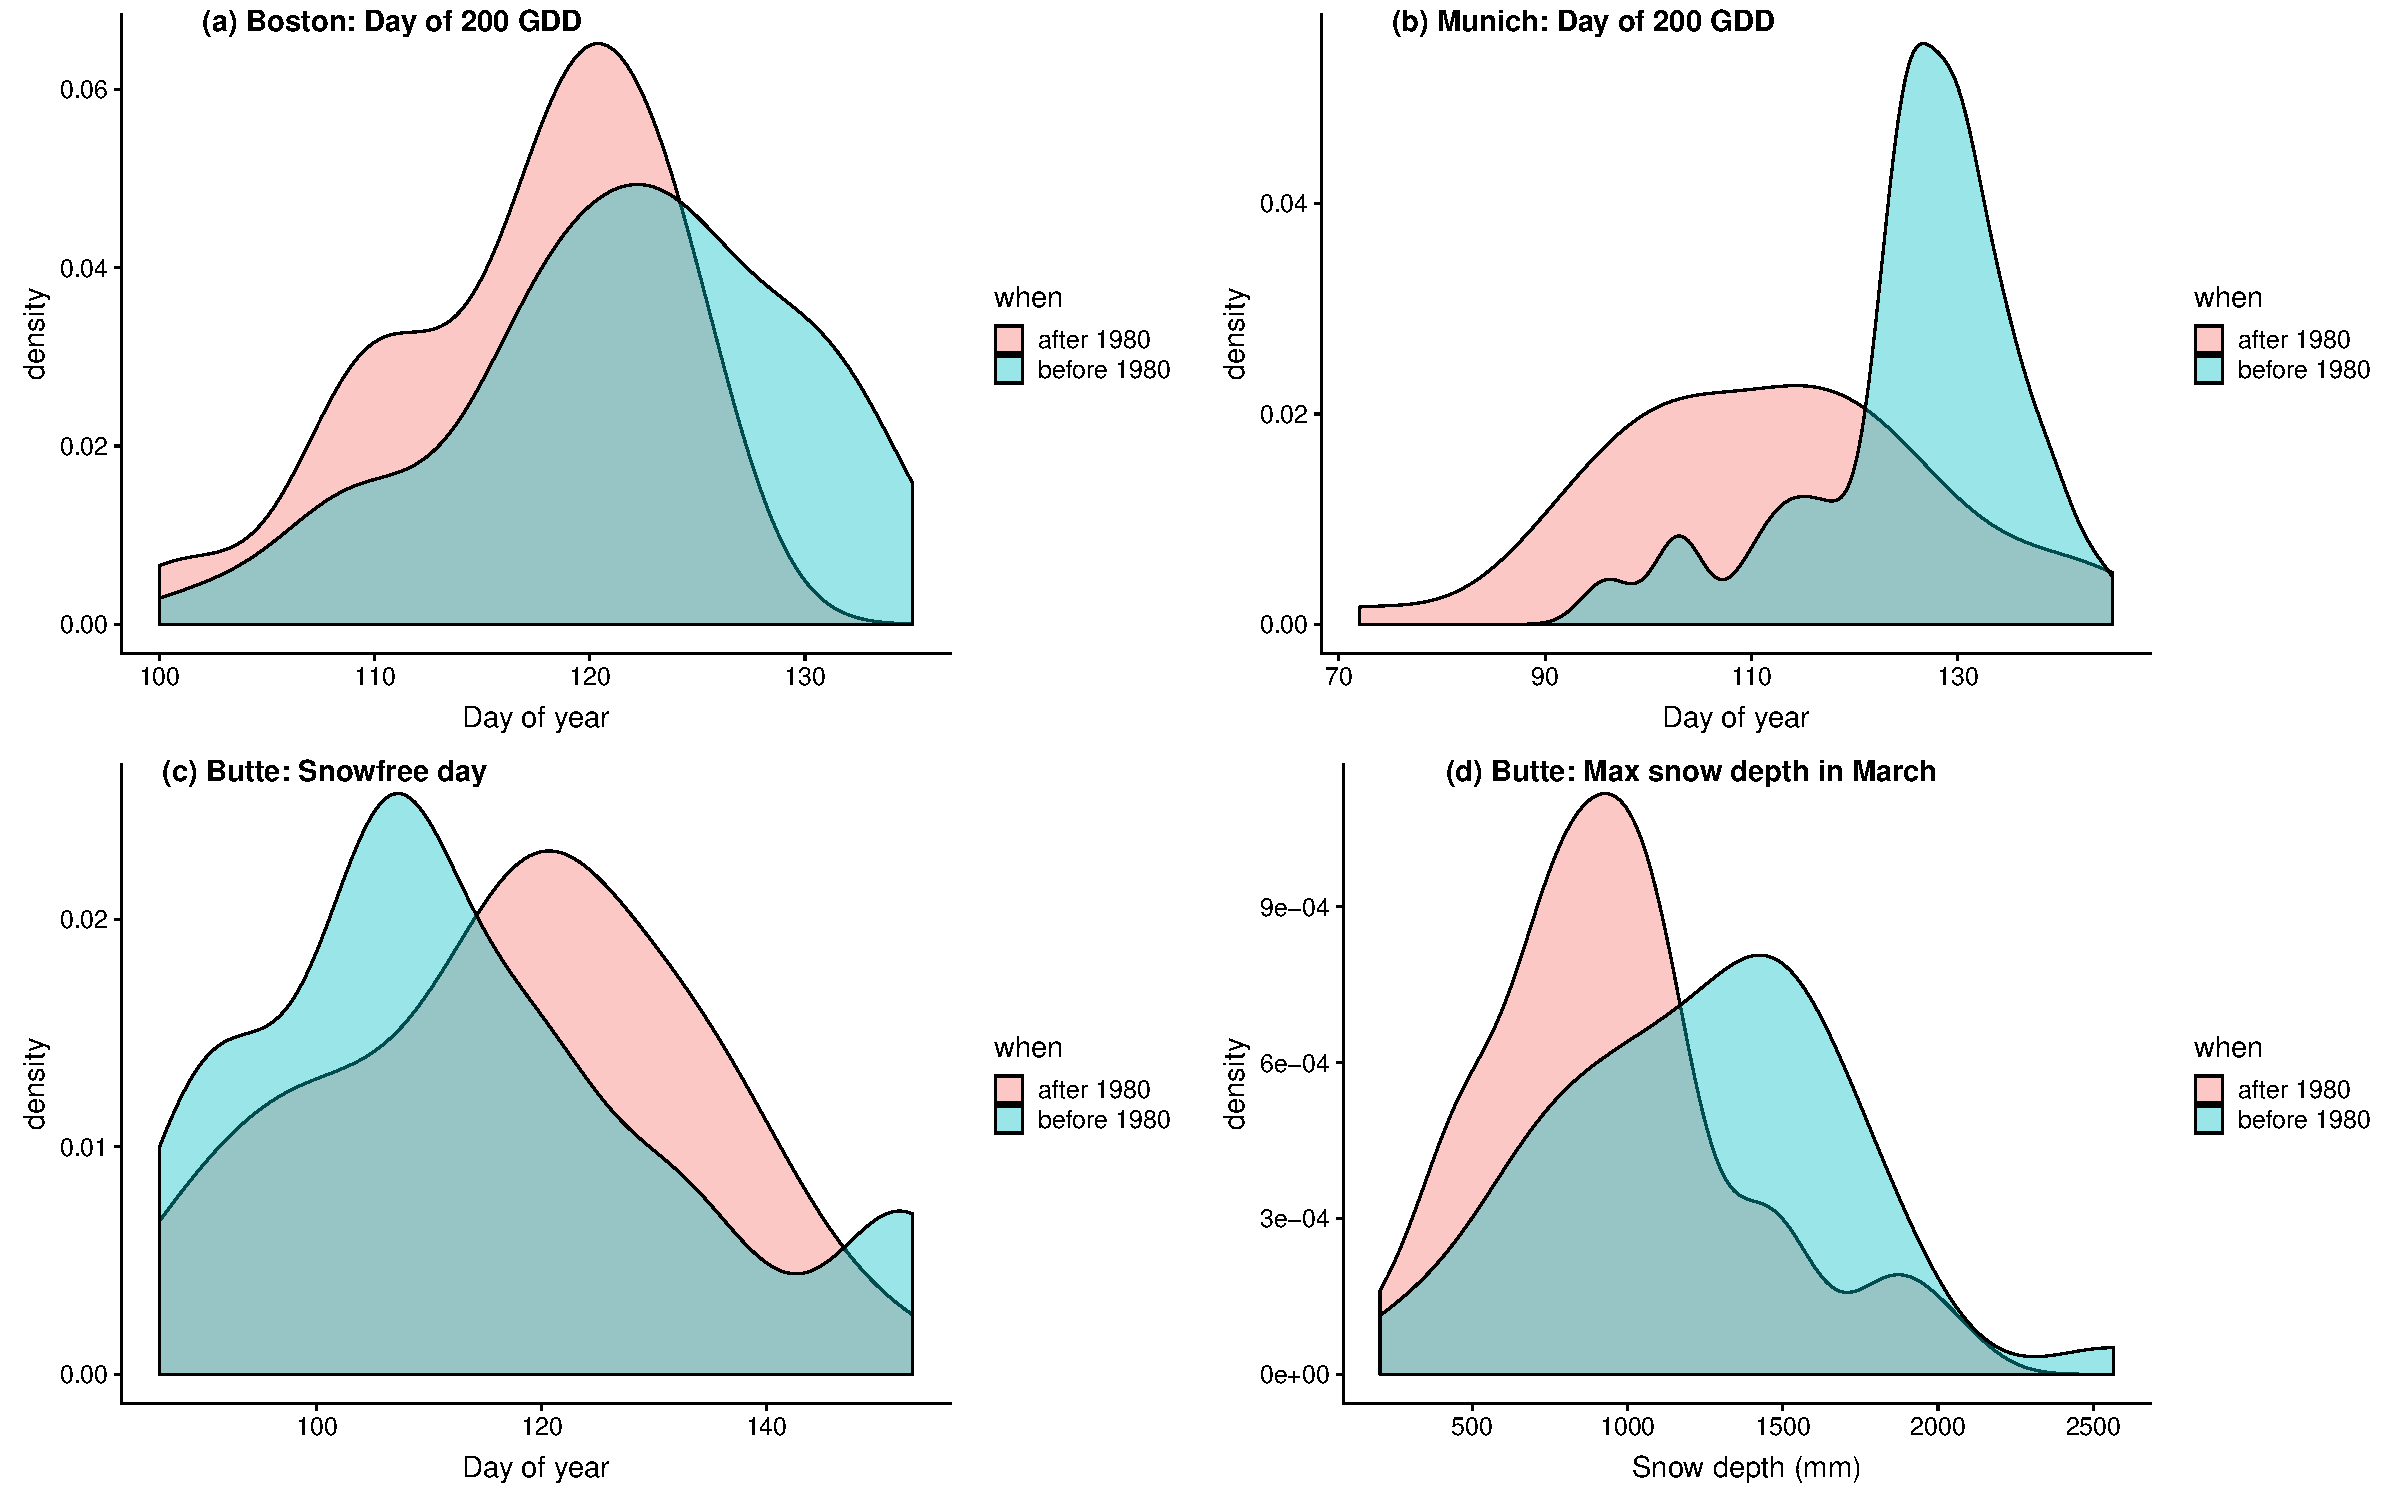
\includegraphics[width=1\textwidth]{..//..//R/graphs/otherdat/climdata.pdf}
\caption{Examples of shifts before and after 1980 (a major changepoint in climate for many regions) in several abiotic metrics related to start of growing seasons (a-c) or resource pulse connected to growing season length (d). Density plots of day of 200 growing degree day units (a metric of themal sum, here based on 0 degree base temperature using daily minima in $\degree$C) in Boston, MA, USA (a), and Munich, Germany (b), first snowfree day (followed by at least 9 snowfree days) in Crested Butte, CO, USA (c) and maximum snowdepth (mm) in March (often the month before the first snowfree day) in Crested Butte, CO, USA (d). Note that (c) and (d) are likely related, with lower snowpacks leading to an earlier first snowfree day. We selected sites that have been studied for plant phenological data and included at least 80 years of daily climate data from a Global Historical Climatology Network site (downloaded from \url{https://climexp.knmi.nl/}); we subsetted data so that there was 40 years before and after 1980 for all sites.}
 \label{fig:climdat}
\end{figure}

\begin{figure}[t!]
\centering
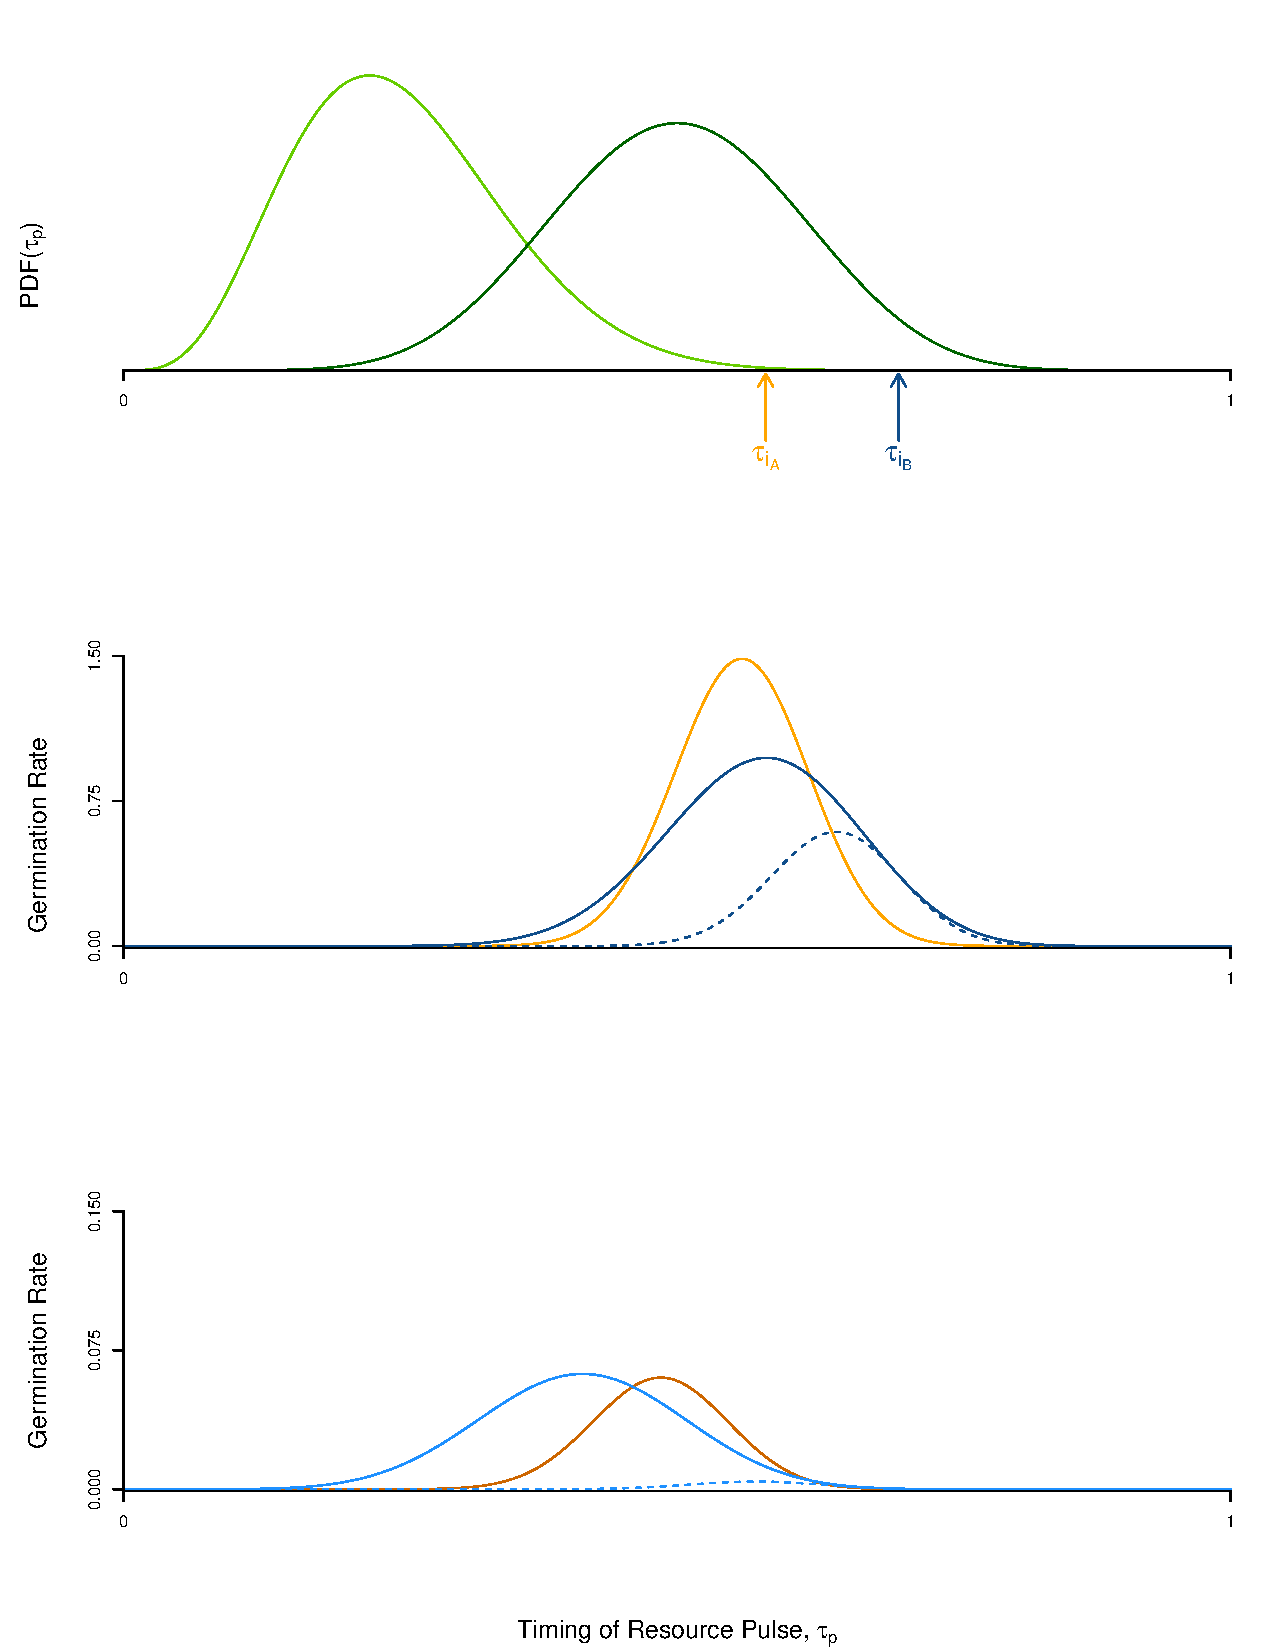
\includegraphics[width=0.9\textwidth]{..//..//figures/TauP_Germination_20190909.pdf} 
\caption{A) The timing of the resource pulse ($tau_P$) is $\beta$-distributed with parameters $\beta(10,10)$ during the stationary period (dark green) shifting to $\beta (5,15)$ through the nonstationary period.  (B) Realized germination rate as a function of $tau_P$ for two species during the stationary period:  the orange line is a non-tracking species A with preferred germination time, $tau_{iA}$ close to the mean of the stationary period; the blue lines show the germination of a tracking species with a preferred germination time $tau_{iB}$ further from the mean of the stationary period both with (solid) and without (dashed) the effect of tracking.  C) Realized germination rate of sp A and sp B at the end of the nonstationary period.  Note the change in axes from (B) to (C) shows the decline in overall germination rate as the environment moves away from the preferred germination time of both species.} % I'm not sure that "realized germiantion" is the best phrase, but it is the germination rate given tauP times the prob of tauP under that STA or NST period.  So it it he realized germination rate for each species given the environment.  
 \label{fig:concept}
\end{figure}

\begin{figure}[t!]
\centering
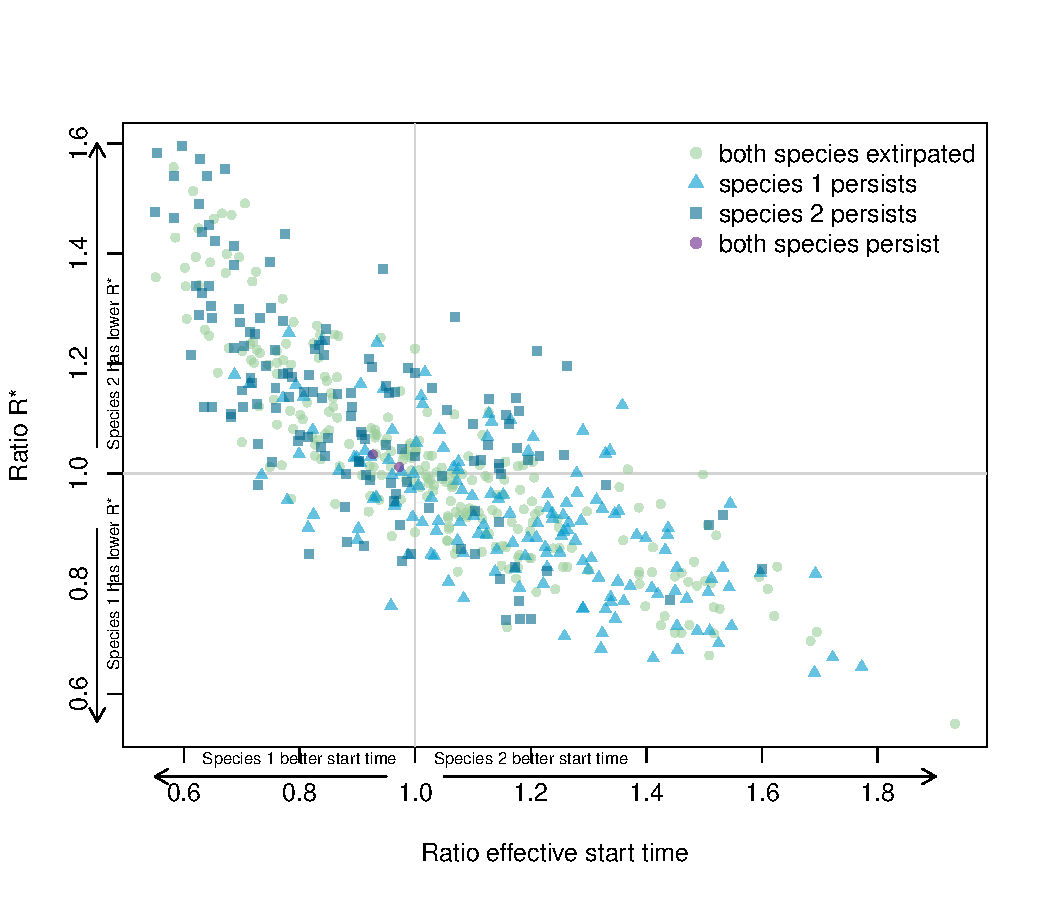
\includegraphics[width=1\textwidth]{..//..//R/graphs/modelruns/manuscript/tauIPrstart1.pdf}
\caption{How non-stationarity reshapes two-species communities in a simple model where effective start time (X axis: species 1/species 2) trades off with $R^*$ (Y axis: species 1/species 2): each point represents one two-species community that persisted through 500 years of stationary dynamics while the shape and color represent the outcome for that two-species community of 500 years of non-stationarity, where the abiotic start of the season shifts earlier.}
 \label{fig:tauirstar}
\end{figure}


\begin{figure}[t!]
\centering
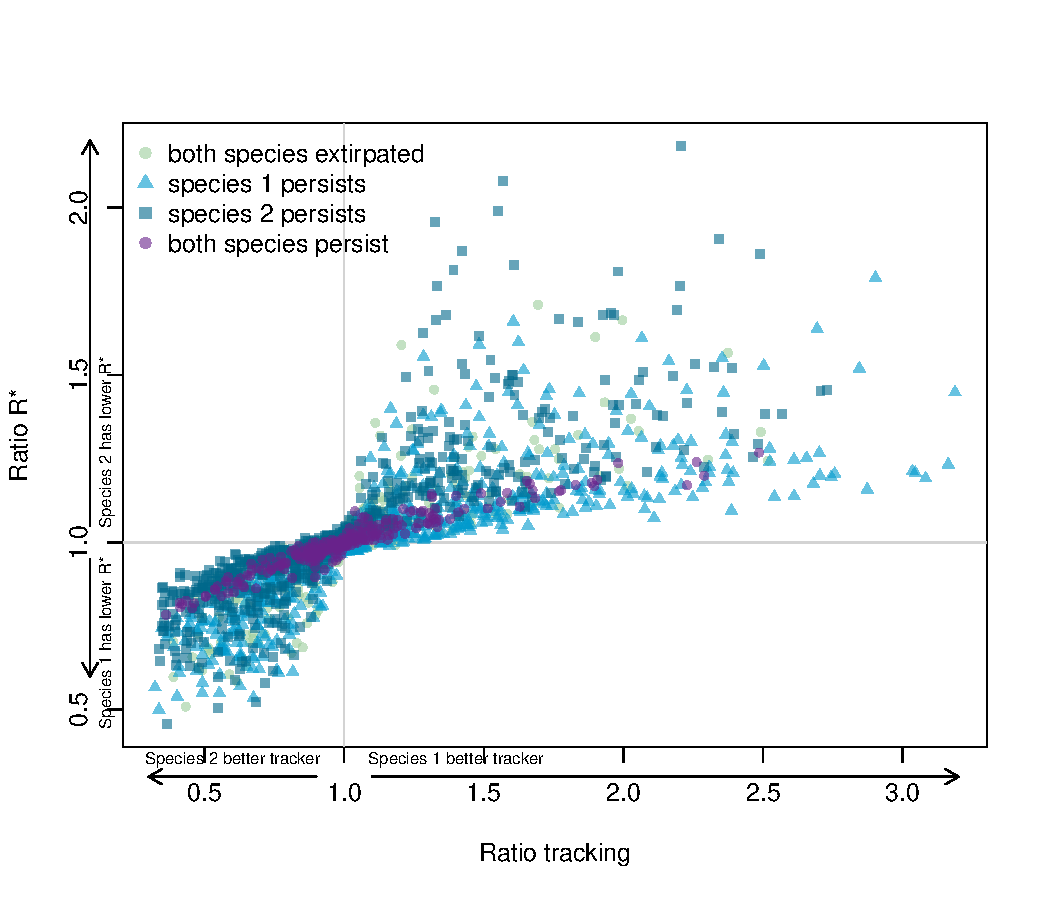
\includegraphics[width=1\textwidth]{..//..//R/graphs/modelruns/manuscript/alpharstar.pdf}
\caption{How non-stationarity reshapes two-species communities in a simple model where tracking (X axis: species 1/species 2) trades off with $R^*$ (Y axis: species 1/species 2): each point represents one two-species community that persisted through 500 years of stationary dynamics while the shape and color represent the outcome for that two-species community of 500 years of non-stationarity, where the abiotic start of the season shifts earlier.}
\label{fig:alpharstar}
\end{figure}


\end{document}
%%%%%%%%%%%%%%%%%%%%%%%%%%%%%%%%%%%%%%%%%%%%%%%%%%%%%%%%%%%%%%%%%%%%%%%%

\section{Figures}
\begin{enumerate}
\item Figure for ... The shape of this underlying distribution varies across systems and in how it is measured---the amount of rainfall in semi-arid systems is often highly skewed compared the thermal sum of many temperate growing season
\item With climate change, warming has increased mean temperatures over time, with minimum temperatures generally increasing mre than maximum---this results in an underlying distribution for daily temperature where the mean is both increased through time and the variance is decreasing (Munich garden? Maybe add San Dieg precip example?
\item Real-world data showing stat/non-stationarity in environment (ideally $\tau_{P}$) 
\item Real-world data showing tracking (and less tracking)
\item $\tau_{i}$ vs. R* trade-off and histogram of persisting $\tau_i$ under stat/nonstat $\tau_{P}$ environment
\item alpha vs.$\tau_i$ trade-off and histogram of persisting alpha under stat/nonstat $\tau_{P}$ environment
\item alpha vs. R* trade-off and histogram of persisting alpha under stat/nonstat $\tau_{P}$ environment
\item (Scratch this one: we're pretty sure it required a crappy $\tau_i$ to survive the initial stationary period, then be favored in second time period and we're not so sure crappy $\tau_i$ species survive the initial stationary period) time-series of one run showing years where $\tau_i$ of one species is close to $\tau_{P}$ and other years where $\tau_i$ of other species is close to $\tau_{P}$ (and show this shift under nonstat)
\item non-stationarity in $R0$ and $\tau_{P}$
\end{enumerate}


%=======================================================================
% to-do listing
%=======================================================================

\listoftodos

%=======================================================================
\section*{Other loose ends}
%=======================================================================

% Old hypothesis: Without tracking we may predict benefits to early-colonizers decline with earlier seasons. As start-date moves earlier, early folks lose benefit (assuming they tend to often go at optimum time) and you get more late folks. Late species may be less different than one another---and less responsive to environment. Early folks, effectively, become more similar to environment. 



% Old parts of intro not currently used....
Athropogenic climate change is causing widespread changes in species, with many species shifting in both time and space (CITES). Many species are shifting in ways predicted by a direct response to track climate---for example, species are shifting up in elevation and poleward as climate warms (CITES), and/or shifting earlier in their recurring life history events (phenology)(CITES). Yet, not all species are shifting as predicted by a simple climate-tracking response; species in the same community can include some that do not shift or even shift in an apparently opposing direction (e.g., delayed spring phenology with warming). \\

Understanding these variable responses of species and communities to climate shifts is a major aim of current ecology and may be explained by indirect effects. Research has already documented changes in a species performance (CITES) and community composition that appear to be---at least in part---indirect effects (CITES).  Understanding ecological responses to climate change will thus require synthesizing information on both direct effects of climate on species and indirect effects driven by responses to other species' shifts. \\ % Alongside these more direct physiological effects of climate change, however, are indirect effects.






